\cotefile{64}
\scanpage{28}
On a

\[
\left\{\begin{aligned}
&M_0\text{ et }\mathbb F_2^{\underline\omega}\text{ sont orthogonaux l'un de l'autre}\\
&\text{dans }\underline{\mathrm{End}}(M_0)\text{ pour la forme }\mathrm{Tr}(uv)
\end{aligned}\right. \tag*{(15)}
\]

\[
\deleted{\unsure{M_0}}\,
\underset{\mathrm{Ker}(\mathrm{End}(M_0)\overset{\mathrm{tr}}{\unsure{\relbar|\to}}\mathbb F_2)}
{\underline{\unsure{\mathfrak{sl}|\mathfrak{gl}}(M_0)}}
=M_0\oplus\mathbb F_2\,\mathrm{id}_{M_0} \tag*{(16)}
\]

\[
\mathbb F_2^{\underline\omega}\cap\mathfrak{sl}(M_0)\simeq
\mathbb F_2\cdot\mathrm{id}_{M_0}\qquad\ldots\qquad\biggr] \tag*{(17)}
\]

Ainsi, la donnée d'un torseur $P_M$ sous $\inserted{V_J(M_0)\simeq}\mathrm{End}(M_0)$ \deleted{\unsure{ou|un}}, équivaut à celle d'un couple de torseurs, \deleted{sous} l'un sous $M_0$, l'autre sous $\mathbb F_2^{\underline\omega}$, soient $I_{\underline M}$ et $S_M$.

\uline{Théorème} Le foncteur \(\displaystyle M\mathrel{\mapstochar\relbar\mapstochar}(\deleted{I}M_0,I_M,S_M)\)

\diagram{\begin{tikzcd}[ampersand replacement=\&,column sep=small]
{(18)} \& {\substack{\mathbb Z/4\mathbb Z\text{-modules}\\ \text{libres de rang }2}}\arrow[r] \& {\text{triplets }(M_0,I_{\deleted{\unsure{M}}},S_{\deleted{\unsure{M}}}).}
\end{tikzcd}}

\deleted{où $M_0$ un vect. de rg $2$} \inserted{avec}

\[
\left\{\begin{aligned}
&M_0\text{ vect. de rg }2\text{ sur }\mathbb F_2\\
&I\quad M_0\text{-torseur}\\
&S\quad\text{torseur sous }\mathbb F_2^{\underline\omega(M_0)}
\end{aligned}\right.
\]

est une équivalence de groupoïdes.

% slanted
\reversemarginpar\margin{\raggedright Équivaut essentiellement à l'isomorphisme $\mathrm{Gl}(2,\mathbb Z/4\mathbb Z)\simeq\overbrace{\mathrm{Gl}(2,\mathbb F_2)}^{\mathfrak S_3}\cdot\mathbb M_2(\mathbb F_2)$ (produit $1/2$ direct), plus l'isomorphisme de $\mathfrak S_3$-modules $(\mathfrak S_3\simeq\mathrm{Gl}(2,\mathbb F_2))$ $\mathbb M_2(\mathbb F_2)\simeq\mathbb F_2^2\times\mathbb F_2^{\underline\omega_0}$, où $\mathrm{Gl}(2,\mathbb F_2)$ opère sur $\mathbb F_2^2$ tautologiquement, et sur $\mathbb F_2^{\underline\omega_0}$ via op. sur $\underline\omega_0$ par signature \ldots\ On a l'inclusion $\mathrm{Sl}(2,\mathbb Z/4\mathbb Z)\unsure{=|\subset|\simeq}\deleted{\unsure{\mathrm{Gl}(2,\mathbb Z/4\mathbb Z)\cdot\mathbb M_2(\mathbb F_2)}}\deleted{\unsure{\mathrm{Gl}(2,\mathbb F_2)\times\mathbb F_2^2\times\mathbb F_2}}\{g\cdot u\in\mathfrak S_3\cdot\mathbb M_2(\mathbb F_2)\mid\mathrm{sg}(g)\,\underline e(\mathrm{Tr}\,u)=1\}$ où $\underline e:\deleted{\unsure{\mathbb Z/2\mathbb Z}}\mathbb F_2\overset{\sim}{\longrightarrow}\{\pm1\}$.}\normalmarginpar

\uline{Corollaire} On a un isom. de suites exactes canoniques ($\forall M$ libre de rg $2$ sur $\Lambda=\mathbb Z/4\mathbb Z$)

\diagram{\begin{tikzcd}[ampersand replacement=\&,column sep=small]
\&1\arrow[r,dash]\&\mathrm{End}_{\mathbb F_2}(M_0)\arrow[r]\&\mathrm{Gl}_{\Lambda}(M)\arrow[r]\&\overset{\simeq\mathfrak S_J}{\mathrm{Gl}(M_0)}\arrow[r,dash]\&1\\
{(19)}\&1\arrow[r,dash]\&M_0\times\mathbb F_2^{\underline\omega}\arrow[u,"\sim"']\arrow[r]\&\mathrm{Aut}(M_0,I_M,S_M)\arrow[u,"\sim"']\arrow[r]\&\mathrm{Gl}(M_0)\arrow[u,equal]\arrow[r,dash]\&1
\end{tikzcd}}

Ici l'hom $\mathrm{End}(M_0)\to\mathrm{Gl}(M)$ est donné par la condition que le composé avec l'hom $\mathrm{End}_{\Lambda}(M)\to\mathrm{End}_{\mathbb F_2}(M_0)$ soit donné par $u\longmapsto\mathrm{id}_M+2u$.
% archive sheet number: 27
\scanpage{29}
\mspage{14}

La \unsure{donnee|donnée} de $(M_0,I)$ équivaut, par le \S~1, à la donnée d'un ens. à quatre éléments $I$, on aura $M_0\simeq V_I$, $M_0^*\simeq\mathcal P_{2,2}(I)$.

\deleted{\unsure{Pour un|Par ailleurs}} \inserted{D'autre} part, \deleted{\unsure{il revient au|à un ens de|la donnée d'un}} \inserted{la donnée d'un} ens à deux éléments $C$, et d'un torseur $S$ sous $\mathbb F_2^C$, équivaut à la donnée d'un carré $Q$, $S$ étant l'ens. des sommets de $Q$, $C$ l'ens de ses codiagonales.

Donc le \deleted{catégorie} \inserted{groupoïde} du deuxième mb de (18) est équivalent aussi à celui des triples $(I,Q;k)$, où $I$ est un ens à quatre éléments, $Q$ un carré, et $k$ un isom.

\[
 k:\underset{\substack{\text{ens des}\\\text{orientations}\\\text{de }I}}{\underline{\underline\omega(I)}}\simeq
 \underset{\substack{\text{ens. des}\\\text{codiagonales}\\\text{de }Q}}{\underline{C(Q)}}. \tag*{(20)}
\]

On trouve donc

\uline{Corollaire 2} On a une équivalence can. de groupoïdes

\[
\underset{\mathbb Z/4\mathbb Z}{\underline\Lambda}\text{-modules }\underset{\text{de rg }2}{\text{libres}}
\xrightarrow{\approx}\text{triplets }(I,Q,k),\quad\text{où} \tag*{(21)}
\]

\[
\left\{\begin{aligned}
&I\quad\text{ens. à }4\text{ élément}\\
&Q\quad\text{carré combinatoire}\\
&k:\underline\omega(I)\simeq C(Q)
\end{aligned}\right.
\]

\uline{Corollaire 3} Si $M$ est associé à $I,Q$, on a un diagramme cartésien canonique

\diagram{\begin{tikzcd}[ampersand replacement=\&,column sep=small]
\&\mathrm{Gl}_{\Lambda}(M)\arrow[dl]\arrow[dr]\&\\
{(22)}\quad\mathfrak S_I\arrow[dr,"\mathrm{sg}"']\&\&\mathcal D_Q\arrow[dl,swap,"{\chi_C\;(\text{opération sur l'ens des codiagonales})}"]\\
\&\{\pm1\}\&
\end{tikzcd}}
% archive sheet number: 28
\scanpage{30}
s'insérant dans le diagramme de suites exactes (auquel il donne naissance)

\diagram{\begin{tikzcd}[ampersand replacement=\&,column sep=0.35em,row sep=0.7em,cramped]
\&\&\&1\arrow[d]\&\&\&\\
\&1\arrow[dr]\&\&\mathfrak S_I^+\times\mathbb F_2^{\underline\omega}\arrow[dl,"\mathrm{pr}_1"']\arrow[dr,"\mathrm{pr}_2"]\arrow[dd]\&\&1\arrow[dl]\&\\
1\arrow[dr]\&\&\mathfrak S_I^+\arrow[dl,Rightarrow]\arrow[dr]\&\&\mathbb F_2^{\underline\omega}\arrow[dl]\arrow[dr,Rightarrow]\&\&1\arrow[dl]\\
{(23)}\&\mathfrak S_I^+\arrow[dr]\&\&\mathrm{Gl}_{\Lambda}(M)\arrow[dl]\arrow[dr]\arrow[dd,"{\text{cart}}" description]\&\&\mathbb F_2^{\underline\omega}\simeq V_{S_Q}\arrow[dl]\&\\
\&\&\mathfrak S_I\arrow[dl]\arrow[dr,"\mathrm{sg}"]\&\&\mathcal D_Q\arrow[dl,"\chi_C"']\arrow[dr]\&\&\\
\&1\&\&\{\pm1\}\arrow[dl]\arrow[dr]\arrow[dd]\&\&1\&\\
\&\&1\&\&1\&\&\\
\&\&\&1\&\&\&
\end{tikzcd}}

\uline{Proposition} Le \inserted{noyau \deleted{\unsure{de}}($\simeq\mathfrak S_I^+$) de l'}hom. canonique $\mathrm{Gl}_{\Lambda}(M)\to\mathcal D_Q$ \deleted{induit un iso} est aussi égal au groupe des commutateurs du sous-groupe \inserted{distingué} $\mathrm{Sl}_{\Lambda}(M)$ d'indice $2$ de $\mathrm{Gl}_{\Lambda}(M)$ (NB $\Lambda^*=(\mathbb Z/4\mathbb Z)^*=\{\pm1\}$), qui est \inserted{donc} d'indice $4$ dans $\mathrm{Sl}_{\Lambda}(M)$ -- le quotient $(\mathrm{Sl}_{\Lambda}(M))_{\mathrm{ab}}$ est \deleted{isomorphe à $\mathbb Z/4\mathbb Z$} \inserted{cyclique d'ordre $4$}, et l'hom

\[
\mathrm{Gl}_{\Lambda}(M)\xrightarrow{\det}\{\pm1\}
\]

est le composé \deleted{\unsure{des deux hom|des hom}}

\[
\mathrm{Gl}_{\Lambda}(M)\longrightarrow\mathcal D_Q
\underbrace{\xrightarrow{\deleted{\unsure{\chi}}\,\det}}_{\substack{\text{noyau }\mathcal D_Q^+,\\\text{cyclique d'ordre }4}}\{\pm1\}. \tag*{(24)}
\]

\uline{Corollaire 1} On a un sous-diagramme de suites exactes de (23), obtenu ainsi :
% archive sheet number: 29
\scanpage{31}
\mspage{\textcircled{15}}

\diagram{\begin{tikzcd}[ampersand replacement=\&,column sep=0.3em,row sep=0.65em,cramped]
\&\&{\deleted{\unsure{1}}}\arrow[dr]\arrow[dr,decorate,decoration={zigzag,amplitude=1.2pt,segment length=3pt}]\&1\arrow[d]\&{\deleted{1}}\arrow[dl]\arrow[dl,decorate,decoration={zigzag,amplitude=1.2pt,segment length=3pt}]\&\&\\
\&1\arrow[dr]\&\&\mathfrak S_I^{\unsure{+|*}}\times\{1,-\mathrm{id}_M\}\arrow[dl,"\mathrm{pr}_1"']\arrow[dr,"\mathrm{pr}_2"]\arrow[dd]\&\&1\arrow[dl]\&\\
1\arrow[dr]\&\&\mathfrak S_I^+\arrow[dl,Rightarrow]\arrow[dr,"{\deleted{\unsure{\searrow}}}"']\&\&\{1,-\mathrm{id}_M\}\arrow[dl]\arrow[dr,"\sim"]\&\&1\arrow[dl]\\
{(25)}\&\mathfrak S_I^+\arrow[dr]\&\&\mathrm{Sl}_{\Lambda}(M)\arrow[dl]\arrow[dr]\arrow[dd,"{\text{cart}}" description]\&\&\{\deleted{\unsure{\mathbb F_2}}1,\underline a_Q\}\simeq\mathbb F_2\arrow[dl]\&\\
\&\&\mathfrak S_I\arrow[dl]\arrow[dr,"\mathrm{sg}"]\&\&\mathcal D_Q^+\arrow[dl]\arrow[dr]\&\&\\
\&1\&\&\{\pm1\}\arrow[dl]\arrow[dr]\arrow[dd]\&\&1\&\\
\&\&1\&\&1\&\&\\
\&\&\&1\&\&\&
\end{tikzcd}}

\uline{Corollaire 2} L'hom can. $\mathrm{Gl}(M)\to\mathcal D_Q$ induit un isomorphisme

\[
\mathrm{Gl}_{\Lambda}(M)_{\mathrm{ab}}=\mathrm{Gl}_{\Lambda}^{\unsure{\prime}}(M)/\mathfrak S_I^+\times
\underset{\substack{\text{Centre de}\\\mathrm{Gl}_{\Lambda}(M)}}{\underline{\{1,-\mathrm{id}_M\}}}
\xrightarrow{\sim}(\mathcal D_Q)_{\mathrm{ab}} \tag*{(26)}
\]

\margin{vectoriel de rang $2$ sur $\mathbb F_2$ et même \uline{can.} isom. à $\mathbb F_2\times\mathbb F_2$}

\reversemarginpar\margin{\uline{NB.} $\left\{\begin{aligned}
\det g&=\deleted{\unsure{\chi_D}}\unsure{\mathrm{sg}|\mathrm{det}|\chi_{\underline\omega}}(\dot g)\\
\mathrm{sg}\,g&=\chi_C(\dot g)\\
\mathrm{det}\,g\cdot\mathrm{sg}\,g&=\chi_D(\dot g)
\end{aligned}\right.$ pour $g\in\mathrm{Gl}(M)$, $\dot g$ im. can $\in\mathcal D_Q$}\normalmarginpar

On peut réunir \inserted{l'essentiel de l'information de} (23) (25) dans un diagramme des sous-groupes de $\mathrm{Gl}_{\Lambda}(M)$, où on a posé pour abréger

\[
\mathfrak z=\{1,-\mathrm{id}_M\}\left(=\mathrm{Cent}(\mathrm{Gl}_{\Lambda}(M))=\mathrm{Cent}(\mathrm{Sl}_{\Lambda}(M))\right) \tag*{(27)}
\]
% archive sheet number: 30
\scanpage{32}
\uline{NB}

\[
\begin{aligned}
\overset{\substack{C_Q\\\rotatebox[origin=c]{90}{$\scriptstyle\simeq$}}}{\underline\omega}&\subset\mathbb F_2^{\underline\omega}=\mathbb F_2^C=V_S\subset\mathcal D_Q&
\underline\omega&=V_S\setminus\mathfrak z_Q&\longleftrightarrow&\ \mathrm{sg}(g)\\
D_Q&\simeq\underline\omega\wedge\underline\mu\subset\mathbb F_2^D=V_A\subset\mathcal D_Q&
\underline\omega\wedge\mu&\simeq V_A\setminus\mathfrak z_Q&\longleftrightarrow&\ \mathrm{sg}(g)\det(g)\\
\underline\omega_Q&\simeq\underline\mu\subset\mathcal D_Q^+\subset\mathcal D_Q&
\underline\mu&\simeq\mathcal D_Q^+\setminus\mathfrak z_Q&\longleftrightarrow&\ \det(g)
\end{aligned}
\]

\[
\begin{aligned}
\text{où}\quad \underline\mu&\unsure{=|\simeq}(\overset{2}{\wedge} M)^*=\mathrm{Or}(M)\\
\mathfrak z_Q&=\{1,\underline a_Q\}=\mathrm{Cent}\,\mathcal D_Q
\end{aligned}
\]

\margin{$\mathrm{Gl}_{\Lambda}(M)'\simeq\mathfrak S_I\times\mathbb F_2\simeq\mathrm{Aut}(\Delta)$ où $\Delta$ est l'octaèdre non orienté associé à $M$ de sommets $\Delta=M^{\unsure{+|*|\#}}/\{\pm1\}$ \ldots}

\diagram{\scriptsize\begin{tikzcd}[ampersand replacement=\&,column sep=0.1em,row sep=1.8em,cramped,execute at end picture={
\draw ([xshift=-4pt]fw.north west) to[out=65,in=230] ($(fw.north west)!0.5!(top.north west)+(-10pt,6pt)$) to[out=60,in=200] ([xshift=-2pt,yshift=5pt]top.north west);
\node[above left] at ($(fw.north west)!0.5!(top.north west)+(-10pt,6pt)$) {$\mathfrak S_{\unsure{I|J}}$};
\draw (vec.north west) to[out=75,in=235] ($(vec.north west)!0.5!(top.west)+(-3pt,0pt)$) to[out=65,in=205] (top.west);
\node[above left,align=center] at ($(vec.north west)!0.5!(top.west)$) {$\mathfrak S_J$\\$\simeq\mathrm{Gl}_{\mathbb F_2}(M_0)$};
\draw ([xshift=4pt]mo.south east) to[out=10,in=230] ($(mo.east)!0.5!(alt.east)+(5pt,-2pt)$) to[out=90,in=245] (alt.south east);
\node[right] at ($(mo.east)!0.5!(alt.east)+(5pt,-2pt)$) {$\mathfrak S_J^+$};
\draw (sl.south east) to[out=-85,in=95] ($(sl.east)!0.5!(alt.east)+(8pt,0pt)$) to[out=-95,in=85] (alt.east);
\node[right,align=left] (quot) at ($(sl.east)!0.5!(alt.east)+(8pt,0pt)$) {$\mathcal D_Q^+\simeq(\mathrm{Sl}_{\Lambda}(M))_{\mathrm{ab}}$\\$\simeq\overset{2}{\wedge}_{\deleted{\unsure{\mathbb Z/4\mathbb Z|\Lambda}}} M$};
\draw (quot.east |- top.north) to[out=-88,in=92] ([xshift=3pt]quot.north east) to[out=-90,in=84] (quot.east |- alt.south);
\node[right] at (quot.east |- sl.south) {$\mathcal D_Q$};
}]
\&\&\&|[alias=top]|{\mathrm{Gl}_{\Lambda}(M)[\simeq\mathfrak S_I\cdot\mathbb F_2^{\underline\omega}]}\&\\
\&\&\mathfrak S_I^+\times\mathbb F_2^{\underline\omega}\arrow[ur,"2"]\&{[\mathfrak S_I\times\mathfrak z]}\arrow[u,dotted]\&|[alias=sl]|{\mathrm{Sl}_{\Lambda}(M)}\arrow[ul,"2"']\\
\&|[alias=vec]|{M_0\times\mathbb F_2^{\underline\omega}\simeq\mathfrak{gl}(M_0)}\arrow[ur,"3"]\&\&\mathfrak S_I^+\times\mathfrak z\arrow[ul,"2"]\arrow[u,dotted]\arrow[ur,"2"]\&\\
|[alias=fw]|{\mathbb F_2^{\underline\omega}}\arrow[ur,"4"]\&\&M_0\times\mathfrak z\simeq\mathfrak{sl}(M_0)\arrow[ul,"2"]\arrow[ur,"3"]\&\&|[alias=alt]|{\mathfrak S_I^+}\arrow[ul,"2"]\\
{(28)}\&\mathfrak z\arrow[ul,"2"]\arrow[ur,"4"]\&\&|[alias=mo]|{M_0}\arrow[ul,"2"]\arrow[ur,"3"]\&\\
\&\&1\arrow[ul,"2"]\arrow[ur,"4"]\&\&
\end{tikzcd}}

\uline{NB} Dans ce diagramme, toutes les flèches sont injectives, et les cinq carrés qui y apparaissent, donc aussi les composés, sont cartésiens. On a marqué sur chaque flèche l'indice \deleted{\unsure{pour}} \unsure{de|pour} l'inclusion de sous-groupes qu'elle représente.

Les iso.

\[
\begin{aligned}
\mathrm{Gl}_{\Lambda}(M)&\simeq\mathfrak S_I\cdot\mathbb F_2^{\underline\omega}\quad(1/2\text{ direct})\quad\text{et}\\
\mathrm{Ker}(\mathrm{sg}\cdot\det)&\simeq\mathfrak S_I\times\deleted{\mathbb F_2}\mathfrak z\quad(\text{prod direct}
\end{aligned}
\]

sont valables quand $M$ est \textquotedblleft $1/2$ déployé\textquotedblright\ i.e. le torseur $P_M$ est trivialisé, alors on a $=$

\[
\mathrm{Gl}_{\Lambda}(M)\simeq
\underbrace{\mathrm{Gl}_{\mathbb F_2}(M_0)}_{\mathfrak S_J}\cdot(M_0\times\mathbb F_2^{\underline\omega})
\simeq\underbrace{(\mathrm{Gl}_{\mathbb F_2}(M_0)\cdot M_0)}_{\mathfrak S_I}\cdot\mathbb F_2^{\underline\omega}
\]

mais ces isom. dépendent du choix d'une trivialisat. de $P_M$ \ldots
% archive sheet number: 31
\scanpage{33}
\mspage{16}
6. \uline{Relation} \uline{avec l'octaèdre non orienté} $\Delta_M$.

Soit

\[
\begin{aligned}
M^*&=\{x\in M\mid x^0\,(\text{image dans }M_0)\ne0\}\\
&=\text{image inverse de }J=M_0^*\subset M_0\text{ par } M\longrightarrow M_0 .
\end{aligned}\tag*{(29)}
\]

\deleted{\unsure{donc on|donc on a}} donc $M^*$ est un torseur relatif sur $M_0^{\unsure{a|*|\#}}=J$, du groupe $(M_0)_J$ (i.e famille constante de groupes isom. à $M_0$, indexée par $J$). Le groupe $(\mathbb Z/4\mathbb Z)^*=\{\pm1\}$ opère sur $M^{*}_{\deleted{\unsure{x|0}}}$, de façon compatible avec la projection $M^*\deleted{\unsure{/\,\{\}|\to}}\to J$, on pose

\[
\Delta_M=M^*/(\mathbb Z/4\mathbb Z)^*=M^*/\{\pm1\}=\mathbb P(M)(\mathbb Z/4\mathbb Z)\tag*{(30)}
\]

ce sont les points \deleted{\unsure{sur}} à val. dans $\Lambda=\mathbb Z/4\mathbb Z$ de la droite projective sur $\Lambda$ définie par $M$, et l'application \deleted{\unsure{canonique}} \inserted{can.}

\[
\Delta_M\longrightarrow J \tag*{(31)}
\]

s'identifie à l'application de restriction, ou réduction mod $2$

\[
\mathbb P(M)(\mathbb Z/4\mathbb Z)\longrightarrow\mathbb P(M)(\mathbb F_2).
\]

C'est une application de degré $2$, qui définit donc sur $\Delta$ la structure de (l'ens. des sommets) d'un octaèdre, \deleted{dont} $J$ est l'ens des diagonales. Les \deleted{Le groupe $\mathrm{Gl}(M)$ opère sur} \inserted{12 arêtes de l'octaèdre sont les} éléments de $\mathcal P_2(\Delta)$ (qui a $\frac{6\cdot5}{2}=15$ éléments) qui ne sont pas \deleted{\unsure{des diago|des diagon|des diagonales}} l'une des trois diagonales, i.e. des trois fibres de (31). Les $8$ faces de l'octaèdre sont les parties à trois éléments $\inserted{f}\deleted{\unsure{Q|D|6}}$ de $\Delta$ telles que l'application induite par (31) soit une bijection

\[
f\xrightarrow{\sim}J\ ; \tag*{(32)}
\]

Elles s'identifient donc aux sections de (31), tandis que les arêtes s'identifient aux sections partielles sur des parties de $J$ à deux éléments, et bien
% archive sheet number: 32
\scanpage{34}
\unsure{entdt|entendu|ent.|ment}) les sommets s'identifient aux sections partielles sur des parties \inserted{de $J$} réduites à un élément -- la relation d'incidence est celle du prolongement des sections, ou encore l'inclusion des parties de $\Delta$.

Le groupe $G=\mathrm{Gl}(M)$ opère sur $\Delta$ par \unsure{autom|automs|automorphismes} d'octaèdre, on voit que $\mathfrak z=\{\pm1\}$ opère trivialement, \deleted{\unsure{d'où}} et $=$ que c'est là le noyau de l'opération, on a donc un hom injectif

\[
\underset{\substack{\rotatebox[origin=c]{90}{$\scriptstyle\simeq$}\\\mathrm{Gl}(M)/\{\pm1\}}}{\mathrm{Gl}(M)'}\longrightarrow\mathrm{Aut}_{\mathrm{oct}}(\Delta)
\]

\reversemarginpar\margin{\uline{NB} $\mathrm{Gl}(M)'\xrightarrow{\sim}\mathrm{GP}(M)$ (groupe projectif \unsure{en|de} \unsure{degré|dim|dimension|rang} $1$)}\normalmarginpar

qui est un isomorphisme, car les deux groupes sont de \deleted{\unsure{ce|un}} même ordre $24\times2=48$, donc on trouve

\[
\underset{\substack{\|\\\mathrm{Gl}(M)/(\mathfrak z=\{\pm1\})\\\rotatebox[origin=c]{90}{$\scriptstyle\simeq$}\\\deleted{\unsure{\mathrm P|\mathrm G}}\mathrm{GP}(M)}}{\mathrm{Gl}(M)'}
\xrightarrow{\sim}\mathrm{Aut}_{\mathrm{oct}}(\Delta)\simeq\mathrm{Aut}^+(\Delta)\times
\underbrace{\{1,\underset{\substack{\downarrow\\\text{antipodisme}}}{\underline a_\Delta}\}}_{\substack{\text{Centre}\\\text{de }\mathrm{Aut}_{\mathrm{oct}}(\Delta)}}
\tag*{(33)}
\]

Le centre de $\mathrm{Gl}(M)'$ \deleted{correspond} \inserted{n'est autre} d'ailleurs que le sous-groupe $\mathbb F_2^{\underline\omega}/\mathbb F_2\cdot\mathrm{id}_{M_0}$ de $\mathrm{Gl}(M)'$ (car le centre de $\unsure{\vert|\prime}\ \mathrm{Gl}(M_0)\simeq\mathfrak S_J$ est nul, donc le centre de $\mathrm{Gl}(M)'$ est contenu dans $\underline{\mathrm{End}}(M_0)/(\mathfrak z=\{\unsure{0_{M_0}|0_M|1_{M_0}},1_{M_0}\})\simeq M_0\times\mathbb F_2^{\underline\omega}/\mathbb F_2$, et s'identifie au sous-groupe des invariants sous $\mathfrak S_J\simeq\mathrm{Gl}_{\mathbb F_2}(M_0)$ de ce groupe, c'est $\mathbb F_2^{\underline\omega}/\mathbb F_2$.

La donnée d'un octaèdre $\Delta$ ayant $J$ comme ens des diagonales équivaut à celle d'un torseur
% archive sheet number: 33
\scanpage{35}
\mspage{17}
sous $\mathbb F_2^J$, que je vais désigner par $P_{M,\Delta}$

\[
 F(\Delta_M)=\underbrace{P_{M,\Delta}}_{\text{ens des faces de }\Delta}
 \quad\text{torseur sous }\mathbb F_2^J\qquad(J=M_0^*) \tag*{(34)}
\]

Or on a

\[
 \mathbb F_2^J\simeq\underset{\substack{\rotatebox[origin=c]{90}{$\scriptstyle\simeq$}\\ M_0}}{V_J(\mathbb F_2)}\times
 \underset{\text{diag}}{\underline{\mathbb F_2}}\tag*{(35)}
\]

et l'opération sur $P_{M,\Delta}$ de l'élément non nul \deleted{\unsure{$\mathbb F_2$}} du facteur $\mathbb F_2$ n'est autre que l'antipodisme. Ceci posé, on a un iso. canonique

\[
 P_{M,\Delta}=F(\Delta_M)\xleftarrow{\sim}P_M/\mathfrak z
 \qquad\underset{\substack{\|\\\text{Centre de }\mathrm{Gl}(M)}}{\mathfrak z}
 =\{\pm\mathrm{id}_M\}\tag*{(36)}
\]

provenant de l’homomorphisme évident

\diagram{\scriptsize\begin{tikzcd}[ampersand replacement=\&,column sep=0.4em]
{\unsure{(|c}}\&P_M\arrow[dd]\&{= \{(\xi_i)_{i\in J}\in M^{*J}\mid \xi_i^0=i\deleted{\unsure{,|k|*}}\ \forall i\in J,\ \sum\xi_i=0\}}\\
{(37)}\&{}\& {(\xi_i)\longmapsto\{(\dot\xi_i)\}\quad\text{où }\dot\xi=\Lambda^*\xi=\pm\xi\in\Delta\text{ pour }\xi\in M^*}\\
\&F(\Delta_M)\&{= \{f\in\mathcal P_3(\Delta_M)\mid \underbrace{f\to J}_{\substack{\text{induit par}\\\Delta\to J}}\text{ bijectif}\}.}
\end{tikzcd}}

Ceci nous montre à nouveau que $\mathrm{Aut}(\Delta_M)\simeq\mathrm{Gl}(M)'$, de façon précise on a l'iso. de suites exactes

\diagram{\scriptsize\begin{tikzcd}[ampersand replacement=\&,column sep=0.35em]
{(38)}\&1\arrow[r]\&\overbrace{\mathrm{End}(M_0)/\mathbb F_2\cdot\mathrm{id}_{M_0}}^{M_0\times\mathbb F_2}\arrow[r]\arrow[d,"\sim"',"{\ast}"]\&\mathrm{Gl}(M)'\arrow[r]\arrow[d,"\sim"']\&\overbrace{\mathrm{Gl}_{\mathbb F_2}(M_0)}^{\mathfrak S_J}\arrow[r]\arrow[d,"\shortparallel"]\&1\\
\&1\arrow[r]\&\underbrace{\mathbb F_2^J}_{\simeq M_0\times\mathbb F_2}\arrow[r]\&\mathrm{Aut}_{\mathrm{oct}}(\Delta_M)\arrow[r]\&\mathfrak S_J\arrow[r]\&1
\end{tikzcd}}

% slanted
\reversemarginpar\margin{\raggedright\uline{NB} La donnée d'un octaèdre (pas orienté) $\Delta$ équivaut à celle d'un couple $(I,\underline\mu)$, où $I$ est un ens. à quatre éléments (l'ens de ses bifaces -- qui définit l'oct. \uline{orienté} correspondant), et où $\mu=\mathrm{or}(\Delta)$ est un ens à deux éléments ; -- mais on \unsure{constate|voit} que (\unsure{puisq.|puisque} $I$ \unsure{donné|de Kant}) la donnée de $\mu$ équivaut à celle \unsure{du|des} \unsure{c/h|cube} $\unsure{C_\Delta|E_\Delta|I_\Delta}$ (cf plus bas), qui est $\simeq\mu\wedge\underline\omega_I$}\normalmarginpar

A un octaèdre $(\Delta,\underline a_\Delta)$ ou $(\Delta\to J)$ sont associés trois ens. à deux éléments remarquables, correspondant aux trois caractères \inserted{non-triviaux} de $\mathrm{Aut}_{\mathrm{oct}}(\Delta)$, i.e. aux trois hom \deleted{\unsure{non}} nuls de \deleted{$\mathrm{Aut}_{\mathrm{oct}}(\Delta)$}

\[
 \mathrm{Aut}_{\mathrm{oct}}(\Delta)_{\mathrm{ab}}\simeq
 (\mathrm{Aut}_{\mathrm{oct}}^+(\Delta)\times\{1,\underline a_\Delta\})_{\mathrm{ab}}
 \simeq\mathbb F_2\times\mathbb F_2
\]

Ce sont respectivement les ensembles
% archive sheet number: 34
\scanpage{36}
\noindent\makebox[0pt][r]{(40)\quad}\(\left\{\begin{minipage}{.44\linewidth}\raggedright\footnotesize
$\deleted{\unsure{\underline\omega_\Delta}}C_\Delta$ (\textquotedblleft \unsure{colors|colours|couleurs}\textquotedblright)
\par ens. des $2$ tétraèdres (échangés par l'antipodisme) inscrits dans le cube qui correspond à $\Delta$

\figure{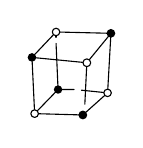
\begin{tikzpicture}[scale=.85,line cap=round,line join=round]
\draw (0,.84)--(.82,.76)--(1.18,1.20)--(.36,1.22)--cycle;
\draw (0,.84)--(.04,0)--(.39,.36)--(.36,1.05);
\draw (.36,1.14)--(.36,1.22);
\draw (.04,0)--(.76,-.02)--(1.13,.31)--(1.18,1.20);
\draw (.82,.76)--(.79,.14);
\draw (.39,.36)--(.63,.36) (.74,.35)--(1.13,.31);
\fill (0,.84) circle (.064) (1.18,1.20) circle (.065) (.76,-.02) circle (.066) (.39,.36) circle (.063);
\draw[fill=white] (.36,1.22) circle (.056) (.82,.76) circle (.058) (.04,0) circle (.057) (1.13,.31) circle (.056);
\end{tikzpicture}}

ou encore des deux couleurs (échangés\ldots) des faces de l'octaèdre $\Delta$

\figure{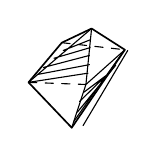
\begin{tikzpicture}[scale=.9,line cap=round,line join=round]
\draw[line width=.6pt] (0,.56)--(.47,1.12)--(.89,1.32)--(1.36,1.02)--(.61,-.08)--cycle;
\draw (.89,1.32)--(.81,.53)--(.61,-.08) (.81,.53)--(1.36,1.02);
\draw[dashed] (0,.56)--(.81,.53) (.47,1.12)--(1.36,1.02);
\draw (0,.56)--(.89,1.32) (0,.56)--(.84,.69) (.12,.67)--(.86,.81)
(.21,.77)--(.86,.94) (.36,.90)--(.87,1.05) (.49,1.01)--(.87,1.16);
\draw (.64,.01)--(1.32,.97) (.69,.14)--(1.23,.80) (.72,.29)--(1.17,.73)
(.78,.42)--(1.10,.66) (1.40,1.01)--(.77,-.05);
\end{tikzpicture}}

correspond au car. \deleted{\unsure{mixte}} de $\mathrm{Aut}_{\mathrm{oct}}^+(\Delta)\times\{1,\underline a_\Delta\}$

\uline{NB} On a $F(\Delta)\simeq\underline C_\Delta\times\underline I_\Delta$ où $I_\Delta=F(\Delta)/\underline a_\Delta$ est l'ens. des quatre directions de faces

\end{minipage}\quad\begin{minipage}{.22\linewidth}\raggedright\footnotesize
$\mathrm{or}(\Delta)$

ens des deux orientations de l'octaèdre $\Delta$

$\simeq$

correspond au car. non trivial de $\{1,\underline a_\Delta\}$

\end{minipage}\quad\begin{minipage}{.22\linewidth}\raggedright\footnotesize
$\deleted{\unsure{C_\Delta\wedge\mathrm{or}(\Delta)}}$
$\underline\omega_\Delta=\underline\omega_{I_\Delta}$

ens. des deux orientations de $I_\Delta$, ou encore, de $J_\Delta$

correspond au caractère non-trivial de $\mathrm{Aut}_{\mathrm{oct}}^+(\Delta)$
\end{minipage}\right.\)

qui satisfont à un iso. canonique

\[
\deleted{\unsure{C_\Delta\wedge}}\mathrm{or}(\Delta)\wedge\underset{\llcorner\mkern-2mu\rule{.85em}{.35pt}\mkern-2mu\lrcorner}{\underline\omega_\Delta}\wedge\underline C_\Delta
\simeq\mathbb 1_{\mathbb F_2}. \tag*{(41)}
\]

On a un isom.

\[
\left\{\begin{aligned}
 C_\Delta&=\bigwedge_{i\in J}\Delta_i\quad\text{quotient de }
 \overbrace{\prod_{i\in J}\Delta_i=F(\Delta)}^{\text{torseur sous }\mathbb F_2^J}\\
 &\text{pour }\underset{\substack{\rotatebox[origin=c]{90}{$\scriptstyle\simeq$}\\\underbrace{V_J(\mathbb F_2)}_{M_0}\times\mathbb F_2}}{\mathbb F_2^J}
 \xrightarrow{\underbrace{(\text{somme})}}\mathbb F_2\\
 \text{i.e.}\quad C_\Delta&=\underbrace{F(\Delta)/M_0}_{} 
\end{aligned}\right. \tag*{(42)}
\]

($P_M/(M_0\times\unsure{\mathfrak z})\deleted{\unsure{\times M_0}}$ dans le cas qui nous occupe) correspond au car. $\mathrm{sg}(g).\det(g)$ dans le cas \deleted{\unsure{qui}} où $\Delta$ est défini par un $M$)

\reversemarginpar\margin{donc dans ce cas on a $C_\Delta\simeq\mu\wedge\underline\omega$}\normalmarginpar

\[
 \underline\omega_\Delta=\underline\omega_{I_\Delta}=\underline\omega_J
 \quad\text{l'ens à deux éléments associé à }J
 \tag*{\deleted{\unsure{(42)}}(43)}
\]

(correspond au caractère $\mathrm{sg}(g)$ dans le cas d'un $M$)

\[
 \deleted{\unsure{\underline\omega}}\mathrm{or}(\Delta)\simeq
 \underset{\underline\omega_J}{\underline{\underline\omega_\Delta}}\wedge C_\Delta \tag*{(44)}
\]

(correspond au caractère $\det(g)$ dans le cas d'un $M$) \unsure{d'où|donc} $\left\lfloor\underline{\mathrm{or}(\Delta)\simeq\mu\overset{\mathrm{def}}{=}(\det M)^*}\right\rfloor$.

L'octaèdre \uline{orienté} \inserted{$\Delta^+$} associé à $M$ est défini par le torseur $P_M/\mathbb F_2^{\underline\omega}$ sous $M_0=V_J(\mathbb F_2)$, i.e. par
% archive sheet number: 35
\scanpage{37}
\mspage{18}
$F(\Delta)/\{1,\underline a_\Delta\}$ (cf (36)), qui est donc l'\unsure{ens|une} des quatre bifaces de $\Delta$. Donc c'est l'octaèdre orienté canoniquement associé à l'octaèdre $\Delta$, savoir

\[
\left\{\begin{aligned}
\Delta^+ &= \deleted{\Delta\wedge_{\unsure{\{1,\underline a_\Delta\}}}}
 \mathrm{or}(\Delta)\wedge_{\{1,\underline a_\Delta\}}\Delta\\
\Delta &= \mathrm{or}(\Delta)\wedge_{\{1,\underline a_\Delta\}}\Delta^+
\end{aligned}\right. \tag*{(45)}
\]

de sorte qu'on a \inserted{bien}, comme il se doit

\[
\left\{\begin{aligned}
\mathrm{or}(\Delta^+) &\simeq \{\pm1\}=\mathbb 1_{\mathbb F_2}\\
\underline\omega_{\Delta^+} &\simeq \underline\omega_\Delta\simeq\underline\omega_J=\underline\omega
\quad [\text{car }\underline a_\Delta\text{ opère trivialement sur }\underline\omega_\Delta]\\
C_{\Delta^+} &\simeq C_\Delta\wedge\mu \simeq \underline\omega\qquad \ldots
\end{aligned}\right. \tag*{(45)}
\]

$[\![$ Il importe maintenant de bien comprendre la structure d'extension

\diagram{\begin{tikzcd}[ampersand replacement=\&,column sep=small,row sep=0pt]
{(47)}\&1\arrow[r] \& \mathfrak z\arrow[r] \& \mathrm{Gl}(M)\arrow[r] \& \mathrm{Gl}(M)'\arrow[r,phantom,"{\unsure{\text{---}|\to}}" description] \& 1\\
\&\& \rotatebox[origin=c]{90}{$\scriptstyle\simeq$} \& \& \rotatebox[origin=c]{90}{$\scriptstyle\simeq$} \&\\
\&\& \{\pm1\} \& \& \mathrm{Aut}_{\mathrm{oct}}(\Delta_M)' \&\\
\&\& \& \& \simeq\mathrm{Aut}_{\mathrm{oct}}^+(\Delta_M)\times\{1,\underline a_\Delta\}_{\unsure{M|\mu}} \&
\end{tikzcd}}

et en particulier

\diagram{\begin{tikzcd}[ampersand replacement=\&,column sep=small,row sep=0pt]
{(48)}\&1\arrow[r] \& \mathfrak z_0\arrow[r] \& \mathrm{Gl}(2,\mathbb Z/4\mathbb Z)\arrow[r] \& \mathrm{Gl}(2,\mathbb Z/4\mathbb Z)'\arrow[r,phantom,"{\unsure{\text{---}|\to}}" description] \& 1\\
\&\& \shortparallel \& \& \rotatebox[origin=c]{90}{$\scriptstyle\simeq$} \&\\
\&\& \{\pm1\} \& \& \mathrm{Aut}'_{\mathrm{oct}}\bigl(\Delta_{\underbrace{(\mathbb Z/4\mathbb Z)^2}_{\substack{\text{\textquotedblleft octaèdre}\\\text{\unsure{standart|standard}\textquotedblright}}}}\bigr) \&
\end{tikzcd}}

puisque c'est par là qu'on comprend quelle est la donnée supplémentaire qu'il faut pour déduire, d'un octaèdre non orienté $\Delta$, le $(\mathbb Z/4\mathbb Z)$-module libre de rang $2$ $M$ dont $\Delta$ proviendrait -- question qui revient à celle de \textquotedblleft remonter\textquotedblright\ un torseur sous le groupe $\mathrm{Gl}(2,\mathbb Z/4\mathbb Z)'$ en un torseur sous le groupe $\mathrm{Gl}(2,\mathbb Z/4\mathbb Z)$ lui-même.
% archive sheet number: 36
\scanpage{38}
Je me \unsure{rapporte|repporte|reporte|reviens} au diagramme (23)

\diagram{\begin{tikzcd}[ampersand replacement=\&,column sep=small,row sep=small]
\& \& \& 1\arrow[dl] \& \&\\
\& \& \mathbb F_2^{\underline\omega}\arrow[dl]\arrow[drr,equal] \& \& \& 1\arrow[dl]\\
\& \mathrm{Gl}_{\Lambda}(M)\arrow[dl]\arrow[dr] \& \& \& \mathbb F_2^{\underline\omega}\simeq V(S_Q)\arrow[dll] \&\\
\mathfrak S_I\arrow[dr] \& \text{cart} \& \mathcal D_Q\arrow[dl,"{\chi_C}"'] \& \& \&\\
\& \{\pm1\}\arrow[dl] \& \& \& \&\\
\unsure{1|\mathfrak z} \& \& \& \& \&
\end{tikzcd}}

qui exprime $\mathrm{Gl}_\Lambda(M)$ comme produit fibré, la donnée de $M$ équivalant à celle du triple $(I,Q,k)$, où $I$ est un ens. à quatre éléments, $Q$ un carré \inserted{combinatoire}, et $k$ un isom

\[
k:\quad\underbrace{C_Q}_{\text{codiagonales}}\quad\overset{\sim}{\rule[.2ex]{1.8em}{.4pt}}\quad\underline\omega_I
\]

En termes de $Q$, on a

\[
 C_\Delta\simeq F(\Delta)/M_0\simeq P_{M,\mathbb F_2^{\underline\omega}}/\mathbb F_2=S_Q/\mathbb F_2\simeq D_Q
\]

ens des diagonales de $Q$ -- donc la donnée de l'octaèdre $\Delta$ (au lieu de $M\longleftrightarrow(I,Q,k)$) équivaut à celle de $I$, et des deux ens. à deux éléments $C$ ($\simeq\omega_I$) et $D$ correspondant aux diagonales et codiagonales du carré $Q$, \deleted{\unsure{ayant|dont|alors que}} la donnée équivaut à celle d'un torseur sous $\deleted{\unsure{\mathcal D_Q}}\mathbb D_4/\mathfrak z(\mathbb D_4)\simeq\deleted{\unsure{\mathbb F_2|\mathbb D_2}}\mathbb F_2\times\mathbb F_2$, qu'il faut donc relever en un torseur sous $\mathbb D_4$. Ou encore, décrire la donnée d'un carré combinatoire, dont on a déjà les deux ensembles \inserted{$C$ et $D$} des codiagonales et diagonales\ldots\ $]\!]$
% archive sheet number: 37
\scanpage{39}
\uline{Récapitulation partielle}

À un module $M$ libre de rang $2$ sur $\mathbb Z/4\mathbb Z$ on associe

\noindent\makebox[0pt][r]{(49)\quad}\(\left\{\begin{minipage}{.77\linewidth}
a) L'octaèdre (non orienté) \inserted{de sommets} $\Delta_M=M^*/\pm1\ \bullet$, l'ens des trois diagonales s'identifiant à $(M/2M)^*\simeq M_0^*=J$

\medskip b) L'ensemble à quatre éléments $I$, qu'on peut p.ex. déduire de $\Delta$ comme
\[
 I_M\simeq\underbrace{F(\Delta)}_{\substack{\text{faces de }\Delta\\\text{i.e. sections de}\\\Delta\text{ sur }J}}/\text{antipodisme}
\]
\end{minipage}\right.\)

\reversemarginpar\margin{On a un iso. can. $J\simeq\mathcal P_{22}(I_M)$, $I_M$ torseur sous $\underset{\simeq\mathbb F_2^J/\mathbb F_2}{\underline{V_J(\mathbb F_2)\simeq M_0}}$ $I_M\simeq P_M/\mathbb F_2^{\underline\omega}$}\normalmarginpar

\margin{\(\left|\begin{array}{ll}\text{\uline{NB}}&F(\Delta)\simeq I\times\underline C_\Delta\\\bullet&\hfill\substack{\downarrow\\\text{\textquotedblleft couleurs\textquotedblright}\\\text{de faces}}\end{array}\right.\)}

\noindent\makebox[0pt][r]{\rule[-1.4ex]{.4pt}{4.6ex}\quad}c) Le carré $Q_M$ \deleted{$\unsure{S_M|S}$} \inserted{ayant comme ens de sommets} $=P_M/M_0$, où $P_M$ est le $\mathrm{End}(M_0)$-torseur formé des sections de $M^*$ sur $M_0^*$ satisfaisant $\unsure{\xi_i+\xi_j+\xi_h|\xi_i+\xi_j+\xi_k}=0$, et où on identifie $\mathrm{End}(M_0)$ à $M_0\oplus\mathbb F_2^{\underline\omega}$, de sorte que $\mathbb P_M/M_0$ est un $\mathbb F_2^{\underline\omega}$ torseur, donc est l'ens des sommets d'un carré \inserted{$Q=Q_M$} dont l'ens des codiagonales est $\underline\omega$

\reversemarginpar\margin{où $\underline\omega\simeq\underline\omega_I\simeq\underline\omega_J$}\normalmarginpar

Les données a) et b) ne dépendent que de la \deleted{fibré} droite projective $X_M=\mathbb P(M)$ sur $\mathbb Z/4\mathbb Z$ ($\Delta$ est l'ens des p\textsuperscript{ts} de celle-ci, $J$ \unsure{celui|celle|c'lui|de l'ens|l'ens} des p\textsuperscript{ts} de $(X_M)_0$ droite projective sur $\mathbb F_2$), mais non pas $Q_M$. On a des bijections canoniques

\[
\left\{\begin{aligned}
\underbrace{C_Q}_{\text{codiag de }Q}&\simeq
\underbrace{\underline\omega_\Delta}_{\deleted{\substack{\text{\unsure{couleurs des}}\\\text{faces de }\Delta}}}
\overset{\text{déf}}{\simeq}\underline\omega_I\simeq\underline\omega_J
&&\text{soit }\underline\omega\\
\underset{\text{diag de }Q}{D_Q}&\simeq
\underset{\text{\textquotedblleft couleurs\textquotedblright\ des faces}}{\underline C_\Delta}
\simeq\underline\omega\wedge\underline\mu
&&\text{où }\underline\mu\ \text{\unsure{défini|définie} ci-dessous}\\
\underset{\text{or. de }Q}{\underline\omega_Q}&\simeq\underline{\mathrm{or}}(\Delta)
\simeq\det(M)^* &&\text{soit }\underline\mu
\end{aligned}\right. \tag*{(50)}
\]
% archive sheet number: 38
